\subsection{Image Classification Setup}

\subsubsection{Dataset}

In this paper we used EMNIST \cite{emnist} data set, which is a collection of handwritten characters and digits from NIST Special Database 19. The data is converted to 28 by 28 matrix so its format matches MNIST data set. There are six subsets in the EMNIST data set: ByClass, ByMerge, Balanced, Letters, Digits and MNIST. We chose the Letter subset because there are around 145k data in it, which will result in a decent running time without loss of information. In the Letter subset, there are 26 classes which corresponding to letter A to letter Z.
\begin{figure}[htp]
    \centering
    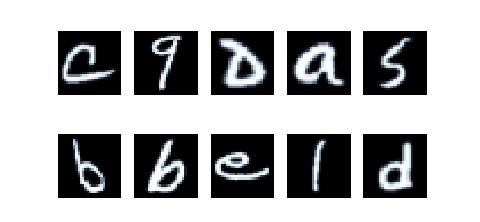
\includegraphics[width=4cm]{img/EMNIST.png}
    \caption{letters in EMNIST}
    \label{fig:EMNIST}
\end{figure}


\subsubsection{Model Architecture}

The first part of the network is a straightforward CNN model and it uses Relu as activation function. It consists of two consecutive convolution layer and pooling layer in order to capture the potential features of the images. The second part of the network flattens the condensed image and then uses two fully connected layer to do the classification.

The cost function is calculated by negative log likelihood loss:
\begin{align*}
    J(y) = -log(y) 
\end{align*}
Note there is only one term in the loss function per data, which is the negative log likelihood of the predicted value of the true label. This negative loss likelihood function works better when the neural network model has a high confidence at the correct class. When training in batch, the cost function per batch is the sum of the individual negative log likelihood costs.

\subsubsection{Evaluation}

The batch size for training is {512, 1024, 2048, 4096, 8192}, the test size is 2048. we keep track of the train loss, test accuracy and test loss for every epoch when using those different optimizers to train the model. For the optimizers, we keep track of the trust ratio and the weight norm of them.


\subsection{Question Answering System Setup}

\subsubsection{Dataset}

For our QA system task, the SQuAD dataset by Rajpurkar et al. \cite{} is employed. There are 80,000 instances for training and 30,000 instance for testing. For each instance, there are question, answers and the context that the question and answer are based on along with the boundary label of the answer. The task is to read the question in order to (1) retrieve the relevant context and (2) then locate the start and end position of the answer. 

\begin{table}[!t]
\vspace{-5pt}
\scriptsize
\vspace{7pt}
\caption{QA System SQuAD examples}\label{tbl:planofwork}
\vspace{-10pt}
\begin{center}
\begin{tabular}{ l|c|c|l}
 \multicolumn{1}{c|}{Context} &
 \multicolumn{1}{c|}{Question} &
 \multicolumn{1}{c|}{Label} &
 \multicolumn{1}{c}{Answer}\\
 %& & \\
\hline
Architecturally, the  & To whom did the Virgin  & [515,  & St Bernadette 
\\
school has a Catholic...  & Mary allegedly appear... & 541] & Soubirous \\ \hline

Architecturally, the  & What is the Grotto  & [381,  & Marian prayer 
\\
school has a Catholic...  & at Notre Dame? & 420] & \& reflection place \\ \hline

Architecturally, the  & What sits on top of the	  & [92,  & a golden statue 
\\
school has a Catholic...  & Main Building at Notre... & 126] & of the Virgin Mary \\ 

\end{tabular}
\end{center}
\vspace{-15pt}
\end{table}


\subsubsection{Preprocessing}

The first transformation for both the question and the context tokens is that they are passed through an embedding layer initialized with pre-trained GloVe word vectors. 100-dimensional vectors from 6B web crawl version are used here. There are 110K vocabularies in total. 


\subsubsection{Model Architecture}

\begin{figure}[!t]
    \centering
    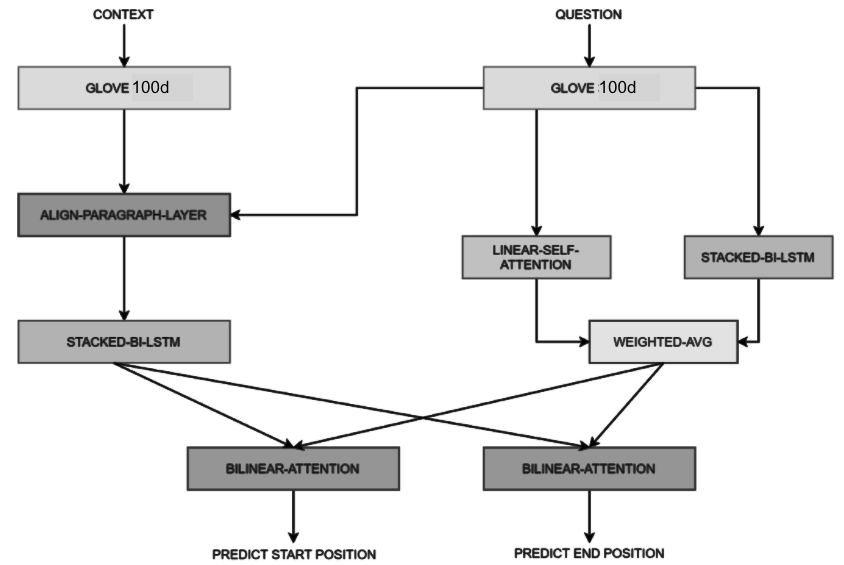
\includegraphics[width=\linewidth]{img/DrQA.png}
    \caption{DrQA model architecture}
    \label{fig:DrQA}
\end{figure}

The model employed for QA end-to-end system here is called Document retriever Question Answering (DrQA) as illustrated in Figure~\ref{fig:DrQA}.  Starting from the top:
\begin{enumerate}
    \item According to Lee et al. \cite{}, the questions and context can be aligned to build respective embedding of: 
    \begin{center} $f_{align} = \sum_j \alpha_{i, j} E(q_j)$. \end{center}
    
    Where $\alpha$ is single dense layer with relu non-linearity and $E()$ represents the glove embeddings. This layer help initialize what portion of the context is more important or relevant with respect to the question.
    
    \item In order to understand the representation of these glove and aligned paragraphs, these are passed to stacked bi-LSTM. 
    
    \item Then the importance of each word in the question is calculated through Linear Attention layer as $b$ below with $w$ as a trainable weight vector:
    \begin{center} 
    $b_j = \frac{e^{w \cdot q_j}}{\sum_{j'}e^{w\cdot q_{j'}}}$
    \end{center}
    
    \item Finally, to predict the accurate answer's span tokens, there are two bilinear classifiers to respectively predict the probabilities of start and end tokens of the span: 
    \begin{center} 
    $P_{start}(i) \propto $
    \end{center}
    
    
\end{enumerate}

% As the name suggested, the model included Document Retriever and Document Reader: 




\subsubsection{Evaluation}

